\section{Our Approach}
\subsection{Aliyun's VM Cloud}
Aliyun provides the largest public VM cloud in China which is based on the 
open-source Xen technology. A typical VM cluster in our cloud environment
consists of from hundreds to thousands physical machines, each of which can
host tens of virtual machines. A few varieties of mainstream OS are supported,
including several editions of Windows Server, major Linux distributions, and FreeBSD.
During the VM creation, user choose his flavor of OS distribution, our system will
copy the corresponding pre-configured base VM image to his VM as the OS disk, 
and an empty data disk is created and mounted onto his VM as well. 

\begin{figure}
  \centering
  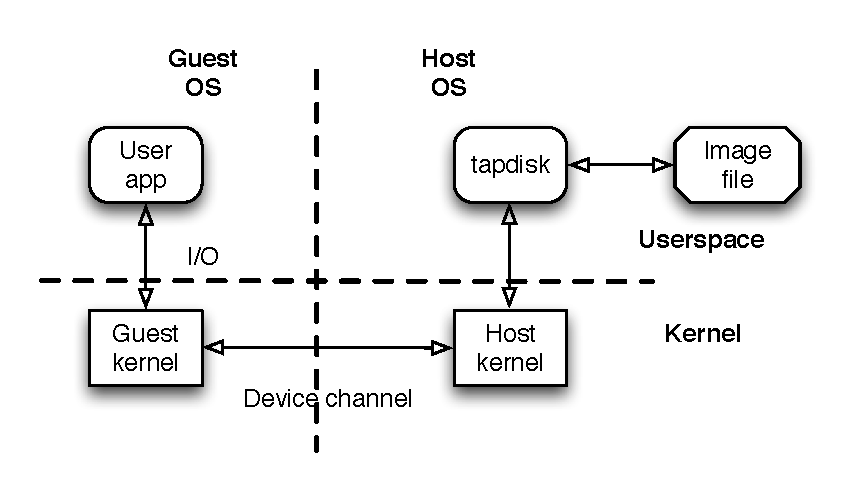
\epsfig{file=images/tapdisk.eps, height=2in, width=2.66in}
  \caption{I/O channel between VM and image files}
  \label{fig:tapdisk}
\end{figure}

All these virtual disks are represented as virtual machine image files in our
underline runtime VM storage system. The runtime I/O between virtual machine and its virtual
disks is tunneled by the TapDisk driver. To avoid network latency and congestion, 
our distributed file system carefully selects the location of primary replica of VM's 
image files such that they are located on the same physical machine of VM instance.

Inside the TapDisk driver, we maintain an array of \emph{dirty bits} to record the dirty area
of runtime VM image file since the last snapshot, each bit represent a 2MB fix-sized
data segment. During a snapshot operation, we only need to look at the dirty region
rather than scan over the whold image file, which would be extremely slow.

The snapshot storage system also resides in our distributed file system, just like the 
runtime VM storage. But the difference is that snapshot storage do not need to be
co-located with VM instances, in fact they can even live in a different cluster to improve the 
data safty. When cluster A is offline, we can quickly restore its VMs from cluster B
to reduce the impact to our users.

The detail design and implementation of our distributed file system and various 
storage subsystems would be too complicated to be intorduced here, and also beyond
the scope of this paper. In the remaining section we will brief the model and interface of 
our snapshot storage.

\subsection{Snapshot Representation}
Each snapshot is a two-level index data structure in the form of HDAG. 
At the bottom level is variable-sized data blocks, like many other deduplication storage systems, 
we use 4KB as the average block size.
In the middle is the segment layer, a segment contains hundreds of blocks, it records the list
of block hash, data reference and some other meta information in a data structure we called
segment recipe. Then the segment recipe itself, can be serialized into a data block, so the hash
of segment recipes and their meta data formed the snapshot recipe. We take this two-level
structure because in practice we observed that at each snapshot only a small fraction
of dirty bits array are marked as set, so snapshot recipes can share the unmodified
segment recipes to reduce the space cost of snapshot meta data.

Instead of using variables-sized segment like many others did, we take the simpler approach
to let every segment being aligned to the boundary of dirty bits array. This is because
\emph{vhd} file format will keep the allocated inner blocks at the same positions until deletion,
which means the locality of snapshot data is almost natively aligned. Enforcing a boundary at every 2MB will
only break 0.2\% of total data blocks which is tiny.

\subsection{Snapshot Storage}
The snapshot storage system sits on top of our distributed file system, 
it can be abstracted as a block store which operates a few \emph{append-only} files
in the underline file storage. Each virtual disk has its own data store, all data 
blocks after deduplication will be stored into that system.

\begin{figure}
  \centering
  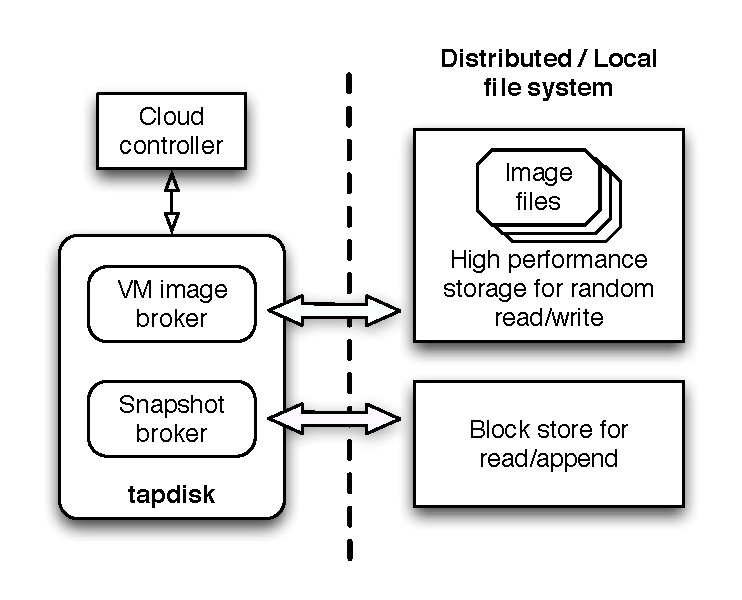
\epsfig{file=images/storage_overview.eps, height=2in, width=2.66in}
  \caption{Storage architecture}
  \label{fig:arch}
\end{figure}

We let each virtual disk has its own block store rather than sharing for several reasons:
first, all data written to block store are already being processed by deduplication
process, thus no sharing is necessary unless we want to perform additional deduplication
inside the block store. Second, such seperation will facilitate VM data stastics, 
deletion and migration. Finally, this reduces the complexity of concurrent snapshot operations.

The main interface of our snapshot storage is \emph{get}, \emph{put} and \emph{delete}.
Get interface accepts a piece of data, write it to the underline data file, and return
a reference to the caller. This reference then can be used in the put interface to
retrive or delete the data, thus the caller of put interface must preserve the
data reference for future use. Since all the underline data structures is append only,
upon a delete request, the corresponding data will only be marked rather than being deleted.
A compaction will take place when deleted data has accumulated to certain threshold, thus 
reclaiming the disk space .

In addition to above data access interfaces, the snapshot storage also supports
\emph{scan} and \emph{quota} methods. Scan allows us to traverse all the data blocks
that store in the data store, and quota is used to acknowledge user how much space he
has actually used.

\subsection{CDS Operations}
The CDS is divided into CDS meta and CDS data. THe structure of CDS meta is not different from the
segment recipe we discussed above, except that it is partitioned into many small slices so that each node
is easy to load its own slice. At the runtime, our CDS meta resides in a global shared memory cache for 
deduplication lookups. The data of CDS is stored in a special block store, which doesn't belong to any VM disk.

CDS meta assignment is done statically, each slice of CDS meta has one primary and two backup nodes.
During the system bootup, snapshot storage controller will read the assignment, 
load its primary portion of CDS meta from distributed file system. Loading the backup portion
of CDS is due upon a query arrives for it. Everyday the CDS assignment and CDS data will be checked
 for updates and reloaded if necessary.

Behind the scene there is a offline map-reduce job, which will periodically scan the block stores
in the entire cluster and perform a ``word counting''. High frequency blocks are then added to the CDS if its count 
 is greater than threshold, which is pre-defined by the system memory restrictions.

\subsection{Dedup Process}
Our deduplication process can be summarized as four steps:
\begin{list}{Dedup}{}
\item {Dirty bits: Copy the unchanged portion of snapshot recipe from parent snapshot, base on dirty bits.}
\item {Locality: Divide dirty segments into blocks, compare to the corresponding segment recipe at the same position of parent snapshot, if duplicate, copy the data reference into segment recipe.}
\item {CDS: Check if this data exist in the CDS, if yes, copy the returned data reference. Otherwise, write data block to block store, save the returned reference into segment recipe.}
\item {Save meta: write down the segment recipes and snapshot recipe when finish.}
\end{list}
